\chapter{Neural Networks and Educational Measurement} \label{ch:irt_background}
In this chapter we present background information for Part I, variational autoencoders for parameter estimation in Item Response Theory. This includes the architecture of particular neural network models, an overview of educational measurement, and a review of other parameter estimation techniques.

\section*{Neural Networks}
In recent years, artificial neural networks (ANN) have become an increasingly popular tool for machine learning problems. Though they have been around since the 1960's \cite{rosenblatt1961}, GPU technology has become more accessible and modern computers are more powerful, allowing any interested researcher to train a basic neural network on a personal machine. ANN can be applied to a diverse set of problems, including regression, classification, computer vision, natural language processing, function approximation, data generation, and more \cite{hammerstrom1993} \cite{zhang2000}. A brief overview of the mathematical inner workings of ANN is included in Appendix \ref{apdx:ann}.

One of the biggest critiques of ANN is their black-box nature, meaning that the decision process of a trained model is typically not explainable by humans. As opposed to simpler methods such as decision trees or linear regression, neural networks are not interpretable. This makes them less desirable in certain applications where researchers wish to know \textit{why} a model outputs a particular prediction in the way that it does. For example, if a financial institution is using data-driven methods to determine whether or not to approve a loan application, the institution should be able to explain to the customer why they were denied \cite{chou2020}. Further, it is possible that a black-box neural network could learn and use sensitive information such as race, age, or gender in its prediction, which would raise legal questions in the United States \cite{ecoa}.

The push for explainable AI has led to multiple approaches to increase model interpretability. Some have aimed to combine deep learning methods with existing interpretable methods, in hopes of increasing the performance of explainable methods without sacrificing its interpretability \cite{goebel2018}. Another option is to use a sort of hybrid learning, where interpretable models defer to a black-box model if they are not confident in their prediction \cite{rafique2020}. Others have started with deep models and cut back on complexity, making specific modifications which increase interpretability. For example, the loss function of a convolutional neural network can be adapted so that humans can better understand the features extracted in the hidden layers \cite{zhang2018interpretable}. 

The field of education is an area which often desires interpretable models. Researchers often need to be able to point out specific details of decisions made by AI. A student deserves an answer to \textit{why} they may have failed a test, and a teacher should be given instructions on \textit{how} to fix the student's misconceptions. 

Part I of this thesis introduces the use of ANN models in educational measurement. A modification is described in Chapter \ref{ch:ml2pvae_methods} which incorporates Item Response Theory and adds interpretability to neural networks. Next, we describe two important types of neural networks -- autoencoders and variational autoencoders -- which can be altered to fit the educational measurement application.

\section{Autoencoders}
An autoencoder (AE) is a neural network where the input and output layers are the same shape. The objective for a given data point is to minimize the difference between the output, called the reconstruction, and the input. Typically, the middle hidden layers of an AE are of smaller dimension than the input space. In this way, autoencoders are an unsupervised learning technique for (nonlinear) dimension reduction. Mathematically, we can define an autoencoder in two parts as follows.

For an input $\vect x \in \R^n$, define the \textit{encoder} as a function $f: \R^n \to \R^d$ mapping $\vect x \mapsto \vect z := f(\vect x)$. Usually, $d < n$, and $\vect z$ lies in a hidden feature space. The encoder sends an observed data point to its representation in a learned feature space. Define the \textit{decoder} as a function $g: \R^d \to \R^n$ mapping $\vect z \mapsto \hat{\vect x} := g(\vect z)$. The decoder maps a hidden representation $\vect z$ to a reconstruction of the original encoder input $\vect x$. Note that in our case, the functions $f$ and $g$ are both parameterized by neural networks, each of which can have any number of hidden layers. The end-to-end autoencoder is then the function composition $\mathcal{A}(\vect x):= g(f(\vect x)): \R^n \to \R^n$, visualized in Figure \ref{fig:ae_visual}.
\begin{figure}[h]
  \centering
  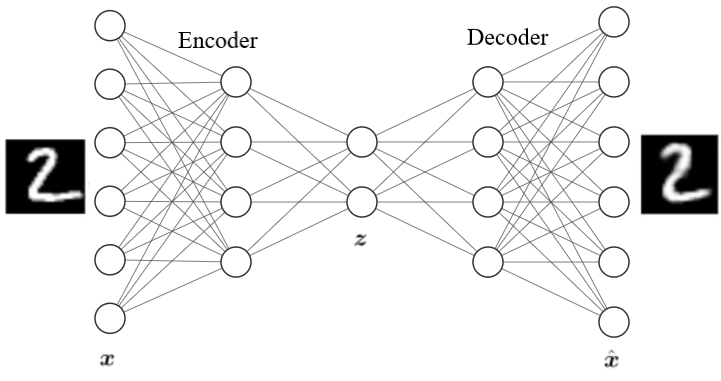
\includegraphics[width=.8\textwidth]{img/ae_visual.png}
  \caption{Visualization of an autoencoder with $n=6$ and $d=2$.}
  \label{fig:ae_visual}
\end{figure}

To train an AE, the loss function minimizes the difference between the input and output (see Appendix \ref{apdx:backprop}). This can be done in a number of ways, including the simple mean squared error loss
\begin{equation}
  \mathcal{L}(\vect x) = || \vect x - g(f(\vect x))||_2^2
  \label{eq:mse}
\end{equation}
or cross-entropy loss for binary data
\begin{equation}
  \mathcal{L}(x) = \sum_{i=1}^n - x_i \log(g(f(x_i))) - (1-x_i)\log(1- g(f(x_i))).
  \label{eq:cross_entropy}
\end{equation}

Autoencoders with only a single hidden layer can be compared with nonlinear principal components analysis (PCA), and using linear activation functions allows for recovery of PCA loading vectors \cite{plaut2018}. AEs have clear applications in image compression straight out-of-the-box, and can be modified for more complicated problems. De-noising autoencoders \cite{vincent2008} are capable of processing noisy images and cleaning them up. To do this, the input data is corrupted by deleting pixels at random. Then, the de-noising AE reconstructs the original image from the corrupted data. Autoencoders can also be modified for data generation applications using a variational autoencoder.



\section{Variational Autoencoders}\label{sec:vae}

The motivation for designing a variational autoencoder (VAE), introduced by Kingma and Welling \cite{kingma2014}, is different from that of a regular autoencoder in that the interest is not rooted specifically to neural networks. Rather, a probabilistic point of view provides the main source of motivation, and ANN are seen as a useful tool used to implement a VAE.

Consider a dataset $\mathbb{X} = \{\vect x_j\}_{j=1}^N$, where each data point $\vect x_j \in \R^n$ is generated by a random process involving an unobserved variable $\vect z \in \R^d$. This unobserved variable is often referred to as ``latent code.'' It is assumed that to generate the observed data point $\vect x_j$, a value $\vect z_j$ is first sampled from a prior distribution $p_*(\vect z)$, and then $\vect x_j$ is generated from a distribution $p_*(\vect x | \vect z)$.

From observing the dataset $\mathbb{X}$, the latent variables $\vect z_j$ and the parameters of the distribution $p_*(\vect x | \vect z)$ are unknown. The goal of a VAE is to approximate these parameters, which leads to the ability to represent the observed data and generate new data. This should be done with a general algorithm that is unaffected by (i) intractability of the marginal likelihood $p(\vect x) = \int p(\vect z) p(\vect x | \vect z) d\vect z$ and (ii) large amounts of data \cite{kingma2014}. Note that (i) is important because if $p(\vect x)$ is intractable and thus $p(\vect z | \vect x)$ is intractable, then the EM algorithm cannot be used -- an issue explored further in Section \ref{sec:em}.

In order to implement this task, two neural networks $q_\alpha(\vect z | \vect x)$ and $p_\beta(\vect x | \vect z)$ (probabilistic encoder and decoder, respectively) are used to approximate the unobservable true posterior distributions $p_{\alpha^*}(\vect z| \vect x)$ and $p_{\beta^*}(\vect x | \vect z)$. In the encoder/decoder, the subscripts $\alpha$ and $\beta$ refer to settings of the trainable parameters of the neural network. Note that unlike a regular autoencoder, the probabilistic encoder $q_\alpha(\vect z | \vect x)$ of a VAE outputs a posterior probability distribution for $\vect z$ given $\vect x$, rather than a single value.

\subsection{A Note on Information Theory}
Before continuing, we introduce some ideas from information theory: entropy, cross-entropy, and KL-Divergence \cite{pattern_rec_book}. Consider a discrete random variable $X$. For a particular value $x$, we can compute the amount of information gained from observing $x$ as $h(X) = -\log_2 p(X=x)$. When we use $\log_2$, the unit for information is ``bits,'' but any base for the logarithm can be used. Note that more information is gained from observing a low-probability event than from observing a high-probability event. 

\textit{Shannon entropy} is defined as the expectation of $h(X)$, or the average amount of information that will be learned by observing a random $x$ when $X$ is a discrete random variable \cite{shannon1948}. The continuous analogue of Shannon entropy is the limiting density of discrete points \cite{jaynes1957}, but is omitted for simplicity. Here, we consider Shannon's \textit{differential entropy} which has a more intuitive formulation, but is a limiting case which lacks the association with discrete entropy. The differential entropy of a continuous random variable $X$ is given as 
\begin{equation}
  H[p] = - \int p(x) \log p(x)dx
  \label{eq:entropy}
\end{equation}

Now assume that we also have access to a distribution $q(x)$ which approximates a possibly unknown $p(x)$. \textit{Cross-entropy} is the average amount of information needed to identify an event $x$ which was drawn from the approximate distribution $q(x)$ instead of drawn from the true distribution $p(x)$. Cross-entropy is given as
\begin{equation}
  H[p,q] = - \int p(x) \log q(x) dx
  \label{eq:xentropy}
\end{equation}

Finally, define \textit{Kullback-Leibler Divergence} (KL-Divergence) \cite{kullback1951} as 
\begin{equation}
  \mathcal{D}_{KL}\left[ p || q \right] = H[p] - H[p,q] = - \int p(x) \log \left(\frac{q(x)}{p(x)} \right)dx
  \label{eq:kl_div}
\end{equation}
Intuitively, KL-Divergence is the average amount of information that is lost if the approximating distribution $q(x)$ is used instead of the true distribution $p(x)$. KL-Divergence cannot be interpreted as a metric or as a distance between the distributions $p(x)$ and $q(x)$ because it is not symmetric -- in general, $\mathcal{D}_{KL}[p||q] \not = \mathcal{D}_{KL}[q||p]$. KL-Divergence is non-negative \cite{kingma2014}, and $\mathcal{D}_{KL}[p||q] = 0$ if and only if $p(x) = q(x)$.

\subsection{VAE Derivation}\label{sec:vae_derive}

We derive the desired loss function for a VAE. The log marginal likelihood of the observed data is given as
\begin{equation}
  \log p_{\beta}(\vect x_1,\ldots,\vect x_N) = \sum_{j=1}^N \log p_{\beta}(\vect x_j)
  \label{eq:vae_marginal}
\end{equation}
Denoting $\vect x = \vect x_j$, we can rewrite each $\log p_{\beta}(\vect x_j)$ term as 
\begin{equation}
  \begin{split}
    \log p_{\beta}(\vect x) &= \int q_\alpha(\vect z |\vect x) \log p_{\beta} (\vect x)d\vect z \\
    &= \int q_\alpha(\vect z | \vect x) \log \left( \frac{p_{\beta}(\vect z | \vect x) p_{\beta}(\vect x)}{p_{\beta}(\vect z | \vect x)} \right) d\vect z  \\
    &= \int q_\alpha(\vect z | \vect x) \log \left( \frac{p_{\beta}(\vect x, \vect z)}{p_{\beta}(\vect z | \vect x)} \right) d\vect z\\
    &= \int q_\alpha(\vect z | \vect x) \left( \log \frac{q_\alpha(\vect z | \vect x)}{p_{\beta}(\vect z | \vect x)} + \log \frac{p_{\beta}(\vect x, \vect z)}{q_\alpha(\vect z | \vect x)}\right) d\vect z \\
    &= \mathcal{D}_{KL}\left[ q_\alpha(\vect z |\vect x) || p_{\beta}(\vect z | \vect x) \right] + \int q_\alpha(\vect z | \vect x) \log \left( \frac{p_{\beta}(\vect x, \vect z)}{q_\alpha(\vect z | \vect x)} \right)d\vect z \\
    &= \mathcal{D}_{KL}\left[ q_\alpha(\vect z |\vect x) || p_{\beta}(\vect z | \vect x) \right] + \mathbb{E}_{q_\alpha(\vect z | \vect x)}\left[ -\log q_\alpha(\vect z | \vect x) + \log p_{\beta}(\vect x, \vect z) \right] \\
    &= \mathcal{D}_{KL}\left[ q_\alpha(\vect z |\vect x) || p_{\beta}(\vect z | \vect x) \right] + \tilde{\mathcal{L}}(\alpha, \beta; \vect x)
\label{eq:vae_derive}
  \end{split}
\end{equation}

Note that in the final line, the first term is the KL-Divergence between the approximate and true posterior. Since we don't know the true posterior, we can't calculate this term. But notice that since KL-Divergence is always positive (i.e. $\forall x \in \R$, $\mathcal{D}_{KL}[p||q] + x \geq x$), it can be ignored and arrive at
\begin{equation}
  \begin{split}
    \log p_\beta (\vect x) \geq \tilde{\mathcal{L}}(\alpha, \beta; \vect x) &= \mathbb{E}_{q_\alpha(\vect z | \vect x)}\left[ -\log q_\alpha(\vect z | \vect x) + \log p_{\beta}(\vect x, \vect z) \right] \\
    &= -\mathcal{D}_{KL}\left[ q_\alpha(\vect z | \vect x) || p_{\beta}(\vect z) \right] + \mathbb{E}_{q_\alpha(\vect z | \vect x)}\left[ \log p_{\beta}(\vect x | \vect z) \right]
  \label{eq:elbo}
\end{split}
\end{equation}

The term $\tilde{\mathcal{L}}(\alpha, \beta; \vect x)$ is referred to as the variational lower bound or Evidence Lower Bound (ELBO). Increasing the ELBO by varying the parameters $\alpha$ and $\beta$ will increase the marginal likelihood $\log p_\beta(\vect x)$, even though we ignore the term $\mathcal{D}_{KL}\left[ q_\alpha (\vect z | \vect x) || p_\beta(\vect z | \vect x) \right]$ in Equation \ref{eq:elbo} \cite{zhao2017}.

We take the ELBO $\tilde{\mathcal{L}}(\alpha,\beta; \vect x)$ to be a potential VAE objective function which we wish to maximize. In Equation \ref{eq:elbo}, the first term gives the negative KL-Divergence between the probabilistic encoder $q_\alpha(\vect z | \vect x)$ and the true prior distribution of the latent code $p_\beta(\vect z)$. Note that unlike the true posterior $p_\beta(\vect z | \vect x)$, the true prior $p_\beta(\vect z)$ is assumed to be known, and it is nearly always assumed to be independent Gaussian. 

For now, we follow suit and assume that $\vect z \sim p_\beta(\vect z) = \mathcal{N}(0,I)$, so we structure the encoder to output a standard normal distribution. In Section \ref{sec:cov}, we propose a novel neural network architecture which generalizes to $\vect z \sim \mathcal{N}(\mu, \Sigma)$ and allows for the encoder to output a multivariate Gaussian distribution.

These assumptions make computing $\tilde{\mathcal{L}}(\alpha,\beta;\vect x)$ much easier. It can be shown \cite{doersch2016} that the KL-Divergence between an independent Gaussian distribution and a standard normal distribution of dimension $K$ is calculated as
\begin{equation}
  \mathcal{D}_{KL}\left[ \mathcal{N}(\vect \mu_0, \vect \sigma_0^2I) || \mathcal{N}(0,I) \right] = \frac{1}{2}\sum_{k=1}^K \left( \mu_k^2 + \sigma_{0,k}^2 - 1 - \log(\sigma_{0,k}^2)\right)
  \label{eq:ind_gauss_kl}
\end{equation}
where the vector $\vect \sigma_0^2$ holds the variances $\sigma_{0,k}^2$ (i.e. the squared standard deviation of each dimension). Note that the vectors $\vect \mu_0$ and $\vect \sigma_0^2$ are outputted by the encoder $q_\alpha(\vect z | \vect x_0)$, given the observed input $\vect x_0$. Since Equation \ref{eq:ind_gauss_kl} is in closed form, there is no difficulty in calculating the (possibly high-dimensional) integral that is usually required to compute KL-Divergence.

The second term in Equation \ref{eq:elbo} is similar to Equation \ref{eq:xentropy}, and depends on the probabilistic decoder $p_\beta(\vect x | \vect z)$, which is usually assumed to be either Gaussian or Bernoulli. Considering the desired application of educational measurement where data is given as binary responses, we assume that the decoder outputs a Bernoulli distribution. To estimate the expectation over $q_\alpha$, we simply sample $L$ times from $q_\alpha(\vect z | \vect x)$. In practice, it is often simplest to just choose $L=1$ \cite{kingma2014}. So then 
\begin{equation}
  \begin{split}
    \mathbb{E}_{q_\alpha(\vect z | \vect x)} \left[ \log p_\beta(\vect x | \vect z) \right] &\approx \frac{1}{L}\sum_{l=1}^L \log p_\beta(\vect x | \vect z^{(l)}) \\
    &\approx \log p_\beta(\vect x| \vect z^*) \\
    &= \log\left( \prod_{i=1}^n p_\beta(x_i = 1 | \vect z^*)^{x_i} \cdot p_\beta(x_i=0 | \vect z^*)^{x_i} \right) \\
  &= \sum_{i=1}^n x_i\log \hat x_i + (1-x_i)\log (1-\hat x_i)
  \end{split}
  \label{eq:bernoulli}
\end{equation}
where $\hat x_i = p_\beta(x_i=1 | \vect z^*)$ gives $\hat{\vect x} = \{\hat x_i\}_{i=1}^n$, the reconstruction of the input $\vect x$ from the encoder $q_\alpha$. Note that the final line of Equation \ref{eq:bernoulli} results in the negative binary cross-entropy loss function commonly used in classification problems.

The process is summarized as follows: given an input vector $\vect x_0 \in \R^n$, we obtain the posterior distribution $q_\alpha(\vect z | \vect x_0)$ (this is done by feeding $\vect x_0$ through the encoder neural network). Sample $\vect z^* \sim q_\alpha(\vect z |\vect x_0)$, and compute $\hat{\vect x} = p_\beta(\vect x | \vect z^*)$ (this is done by feeding $\vect z^*$ through the decoder neural network). As demonstrated in Equation \ref{eq:ind_gauss_kl} and Equation \ref{eq:bernoulli}, we can easily compute each term of the objective function $\tilde{\mathcal{L}}(\alpha, \beta; \vect x_0)$.

Usually when working with neural networks, the goal is to minimize a loss function, rather than maximize an objective function. As such, we define the loss function 
\begin{equation}
  \label{eq:vae_loss}
  \begin{split}
  \mathcal{L}&(\alpha, \beta; \vect x) = - \tilde{\mathcal{L}}(\alpha, \beta;\vect x) \\
  &= \Big(\sum_{i=1}^n - x_i\log p_\beta(x_i | \vect z^*) - (1-x_i)\log (1-p_\beta(x_i | \vect z^*)) \Big) + \mathcal{D}_{KL}\left[ q_\alpha(\vect z | \vect x) || p_\beta(\vect z) \right]
  \end{split}
\end{equation}
where $\vect z^* \sim p_\beta(\vect z) = \mathcal{N}(0,I)$. The parameters $\alpha$ and $\beta$ represent the weights and biases of the encoder and decoder, and are updated via a gradient descent algorithm in order to minimize $\mathcal{L}(\alpha, \beta; \vect x)$ given in Equation \ref{eq:vae_loss}. Note that $\mathcal{L}(\alpha, \beta; \vect x)$ can simply be understood as reconstructing a binary input $\vect x$ via the first term (which mirrors the binary cross-entropy loss function in Equation \ref{eq:cross_entropy}), while regularizing on the latent code $\vect z$ via the second term.


\subsection{Implementation Details}
Recall that each observed data point $\vect x_j \in \R^n$ and the corresponding latent code $\vect z_j \in \R^d$. To parameterize the encoder $q_\alpha(\vect z | \vect x)$ as a neural network, an input layer with $n$ nodes is required. The encoder can (but does not need to) include a number of hidden layers of varying size. The output of the encoder must include $2\cdot d$ nodes, assuming that $p_\beta(\vect z) = \mathcal{N}(0,I)$. 

Notice that in Equation \ref{eq:ind_gauss_kl}, there is a term $\log(\sigma_{0,k}^2)$, dependent on input $\vect x_0$ and all parameters of the encoder. If $\sigma_{0,k}^2 \leq 0$ at any point during training for any $k$, then the VAE loss would not be possible to calculate. To avoid this issue and ensure that $\sigma_{0,k}^2 > 0$ regardless of inputs or encoder parameters, the encoder outputs the log-variances rather than the variances. The first $d$ nodes outputted by the encoder represent the latent mean vector $\vect \mu$, and the last $d$ nodes represent the $\log$ latent variances $\log \vect \sigma^2$. So for an observed input $\vect x_0$, the encoder will output a $d$-dimensional standard normal distribution $\mathcal{N}(\vect \mu_0, \vect \sigma_0^2I)$.

The input layer of the decoder $p_\beta(\vect x | \vect z)$ has $d$ nodes and takes in a sample from $\mathcal{N}(\vect \mu_0, \vect \sigma_0^2I)$, given the original input $\vect x_0$. But the sampling operation is not deterministic, posing a problem for backpropagation-based gradient descent. A re-parameterization is used: sample $\vect \e_0 \sim \mathcal{N}(0,I)$, then calculate $\vect z_0 = \vect \mu_0 + \vect \e_0 \odot \vect \sigma_0^2$ where $\odot$ is element-wise vector multiplication. Then $\vect z_0$ is fed through a number of hidden layers to an output layer of size $n$. The output can be interpreted as the reconstruction $\hat{\vect x_0}$.

\begin{figure}[h]
  \centering
  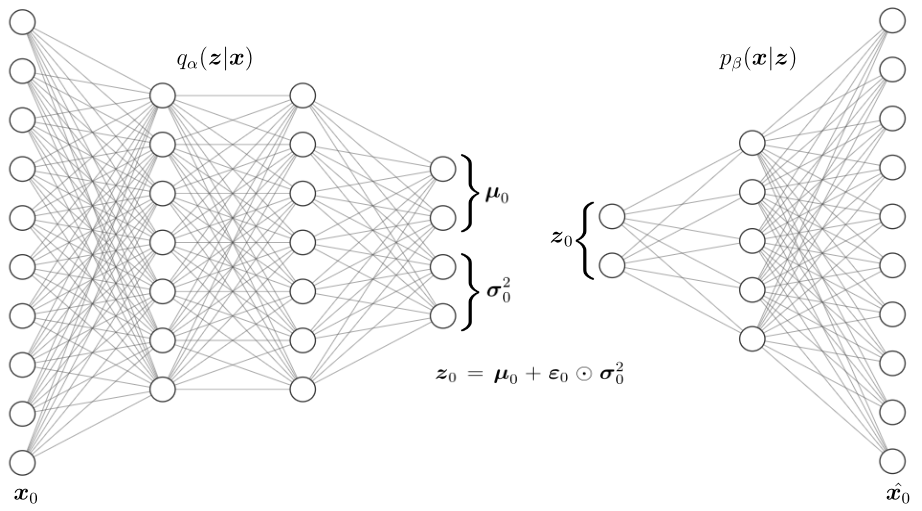
\includegraphics[width=.95\textwidth]{img/vae_visual.png}
  \caption{Visualization of a VAE architecture with $n=10$ and $d=2$.}
  \label{fig:vae_visual}
\end{figure}
The VAE architecture is summarized in Figure \ref{fig:vae_visual}. Note that the VAE does not need to be symmetric -- the encoder and decoder can have a different number of hidden layers of different sizes.


\section*{Educational Measurement}
In educational measurement, a common goal is to quantify the knowledge of students from the results of some assessment. In a classroom setting, grades are typically assigned based on the percentage of questions answered correctly by a student on assignments. The letter grades assigned from these percentages can serve as a naive measure of student knowledge -- ``A'' students have completely mastered the material, ``B'' students have a good grasp of material, ``C'' students are fairly average, and ``D'' and ``F'' students have significant gaps in their knowledge.

The practice of evaluating student ability purely from a raw percentage score is known as classical test theory (CTT) \cite{thissen}. But there are clear issues with this approach. Not all questions on an exam or homework assignment are created equally -- some questions are easier, and some more difficult. Consider a scenario where two students both answer 17 out of 20 questions correctly on a test for a raw score of $85\%$. But if Student A answered questions 1, 8, and 9 wrongly while Student B answered 4, 17, and 20 incorrectly, it is not likely that that Student A and Student B possess the same level of knowledge. For example, questions 1, 8, and 9 could be much more difficult than questions 4, 17, and 20, or Student B may have guessed correctly on some items. Additionally, the two sets of problems could cover different types of material. CTT does not account for either of these situations, and naively quantifies the knowledge of Student A and Student B as equal.

More sophisticated methods have been developed which attempt to more accurately quantify student learning. Cognitive Diagnostic Models (CDM) aim to classify whether students possess mastery of a given skill or not \cite{sinharay2007}. This discrete classification can be useful in determining whether or not a student meets a prerequisite, or in deciding if the student is proficient enough to move on to the next level of coursework. We focus instead on Item Response Theory, where student knowledge is assumed to be continuous. In this case, a student's latent ability is quantified as a real number lying within some interval, such as $(-3,3)$. A value near the middle of the interval translates to a student with average knowledge, and a large (resp. small) value corresponds with a high (resp. low) level of understanding.

\section{Item Response Theory}\label{sec:irt}
Item Response Theory (IRT) is a field of quantitative psychology which uses statistical models to model student knowledge \cite{lord1968}. These models often give the probability of a question being answered correctly as a function of the student's ability. In IRT, it is assumed that each student, indexed by $j$, possesses some continuous latent ability $\theta_j$. The term ``latent ability'' is synonymous with ``knowledge,'' ``trait,'' or ``skill.'' Often, it is assumed that amongst the population of students, $\theta_j \sim \mathcal{N}(0,1)$ \cite{thissen}. 

In this work, we often consider the multidimensional case where each student has multiple latent abilities. For example, in the context of an elementary math exam, we may wish to measure the four distinct skills ``add'', ``subtract'', ``multiply'', and ``divide.'' This scenario is referred to as multidimensional item response theory, and we write the set of student $j$'s $K$ latent abilities as a vector $\vect \Theta_j = (\theta_{1j}, \theta_{2j}, \ldots, \theta_{Kj})^\top$. It is then assumed that the latent abilities of students follow some multivariate Gaussian distribution, $\mathcal{N}(0, \Sigma)$. For simplicity, the covariance matrix $\Sigma$ is often taken to be the identity matrix, making each latent skill independent of one another. This assumption on $\Sigma$ gives practical advantages in estimation, but is often not realistic in real-world applications.

Note that $\vect \Theta_j$ is not directly observable in any way. Given a student's responses to an assessment with $n$ items, a common task is to infer their knowledge $\vect \Theta_j$. Student $j$'s set of responses can be written as a binary $n$-dimensional vector $\vect u_j = (u_{1j}, u_{2j}, \ldots, u_{nj})^\top$, where 
\begin{equation}
  u_{ij} = \begin{cases} 1 & \text{if student } j \text{ answers item } i \text{ correctly} \\0 & \text{otherwise} \end{cases} 
  \label{eq:responses}
\end{equation}
IRT models aim to model the probability of a student answering a particular question correctly, so that the probability of student $j$ answering item $i$ correctly is given by some function of $\vect \Theta_j$:
\begin{equation}
  P(u_{ij} = 1 | \vect \Theta_j) = f(\vect \Theta_j; V_i)
  \label{eq:item_response_prob}
\end{equation}
where $V_i$ is a set of parameters associated with item $i$. In general, $f:\R^K \to [0,1]$, where $K$ is the number of latent abilities, a continuous function which is strictly increasing with respect to $\vect \Theta_j$. Often, the function $f$ follows a curve similar to what is shown in Figure \ref{fig:icc}.

\begin{figure}[h]
  \centering
  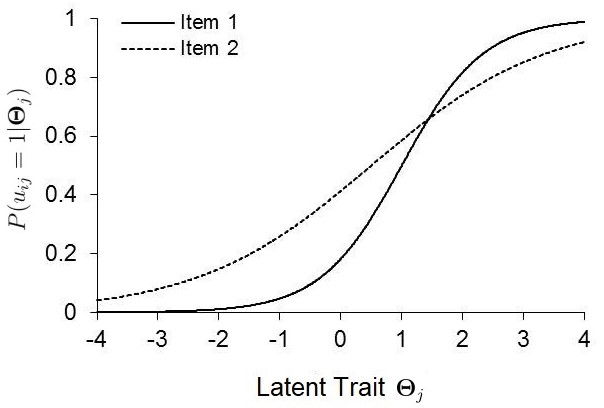
\includegraphics[width=.6\textwidth]{img/logistic_2param_icc.jpg}
  \caption{An item characteristic curve visualizes the relation between a student's ability and the probability of answering an item correctly.}
  \label{fig:icc}
\end{figure}

It is worth mentioning that IRT models also exist for non-binary response data. For example, Samejima's graded response model \cite{samejima1997} allows for items to be answered in multiple categories or grades. This idea is related to partial credit scoring \cite{masters1982}, where students can receive a fraction of the points available on a single question if they demonstrate some knowledge of how to answer the question correctly. In this case, $u_{ij}$ could hold the possible values $\{0, \frac{1}{4}, \frac{1}{2}, \frac{3}{4}, 1\}$, and Equation \ref{eq:item_response_prob} could be characterized as 
\begin{equation}
\begin{split}
  P(u_{ij} \geq 0 | \vect \Theta_j) &= 1 \\
  P(u_{ij} \geq \frac{1}{4} | \vect \Theta_j) &= f_1(\vect \Theta_j;V_i) \\
P(u_{ij} \geq \frac{1}{2} | \vect \Theta_j) &= f_2(\vect \Theta_j;V_i) \\
P(u_{ij} \geq \frac{3}{4} | \vect \Theta_j) &= f_3(\vect \Theta_j;V_i) \\
P(u_{ij} = 1 | \vect \Theta_j) &= f_4(\vect \Theta_j;V_i) 
\end{split}
  \label{eq:graded_response_prob}
\end{equation}

In the following sections, we describe various candidates for the function $f$. The focus is on dichotomous responses as in \ref{eq:responses}, but can be extended to the graded response model. Though each is presented in the context of single-dimensional IRT ($K = 1$), they can all be easily adapted to higher dimensions where $\vect \Theta_j$ is a vector.

\subsection{Rasch Model}
One of the first IRT models was proposed by Georg Rasch in 1960 \cite{rasch1960}. Rasch asserted that the probability of a student answering an item correctly is a function of the ratio $\xi / \d$, where $\xi > 0$ represents the student's knowledge, and $\d > 0$ quantifies the difficulty of an item. Consider the value $\displaystyle \frac{\xi}{\xi + \d} = \frac{1}{1 + \d / \xi}$ and note that $\displaystyle \frac{\xi}{\xi + \d} \to 1$ as $\xi \to \infty$. After the re-parameterization $\xi = e^{\theta}$ and $\d = e^{b}$, we arrive at the 1-Parameter Logistic Model, often referred to as the Rasch Model \cite{thissen}.
\begin{equation}
  \begin{split}
    P(u_{ij} = 1 | \xi_j; \d_i) &= \frac{1}{1 + \displaystyle \d_i/\xi_j} = \frac{1}{1 + \displaystyle e^{b_i}/e^{\theta_j}} \\
  P(u_{ij} = 1 | \theta_j; b_i) &= \frac{1}{1 + e^{b_i - \theta_j}} 
  \end{split}
  \label{eq:rasch}
\end{equation}

Note that $\theta \in \R$ and $b \in \R$ still represent student ability and item difficulty, respectively. We can interpret the difficulty parameter $b$ as a threshold: when $\theta = b$, then the student has a $50\%$ chance of answering the question correctly. The plot shown in Figure \ref{fig:icc}, the item characteristic curve (ICC) of two items are shown. The role of the difficulty parameter $b_i$ is to transpose the curve to the left (for an easier item) or to the right (for a more difficult item). The slope of the ICC is unaffected by the difficulty parameter.


\subsection{Normal Ogive Model}\label{sec:ogive}
A slightly more sophisticated method for measuring student performance is the normal ogive model. We introduce a discrimination parameter, $a_i$, which quantifies the capability of item $i$ in distinguishing between students who have or have not mastered the knowledge concept $\theta$ \cite{thissen}. In other words, $a_i$ tells \textit{how much} of skill $\theta$ is required to answer item $i$ correctly. The effect of different quantities of $a_i$ is seen in Figure \ref{fig:icc} -- the curve for Item 1 has a steeper slope than that of Item 2, due to Item 1 having a larger discrimination parameter than that of Item 2.

The normal ogive model give the probability of student $j$ answering item $i$ correctly as
\begin{equation}
  P(u_{ij} = 1 | \theta_j; a_i, b_i) = \frac{1}{\sqrt{2\pi}} \int_{-a_i \theta_j + b_i}^\infty e^{\frac{-z^{2}}{2}}dz
  \label{eq:ogive}
\end{equation}
Note the similarity between Equation \ref{eq:ogive} and the cumulative distribution function for a Gaussian distribution. The normal ogive model is popular among statisticians for this reason, but can be difficult to use for parameter estimation due to its complicated form.

\subsection{2-Parameter Logistic Model}
The model which this work focuses on most is the 2-parameter logistic (2PL) model. Like the normal ogive model, the 2PL model uses both the discrimination and difficulty item parameters. The probability of student $j$ answering item $i$ correctly is given by
\begin{equation}
  P(u_{ij} = 1 | \theta_j; a_i, b_i) = \frac{1}{1 + e^{-a_i \theta_j + b_i}}
  \label{eq:2PL}
\end{equation}
Equation \ref{eq:2PL} has the same form (a logistic curve) as that of the Rasch model in Equation \ref{eq:rasch}, but adds in the discrimination parameter $a_i$ which serves the same purpose as the discrimination parameter of the normal ogive model in Section \ref{sec:ogive}. If this parameter is scaled by 1.7, then the ICC from the normal ogive model differs from that of the 2PL model by $0.01$ uniformly \cite{baker_kim2004}. In a sense, we can consider the 2PL model to be a very good approximation of the normal ogive model. Due to the simple form of Equation \ref{eq:2PL}, using this model makes parameter estimation much easier than the normal ogive model.

\subsection{Multidimensional Item Response Theory}\label{sec:mirt}
The previously described statistical models can all be extended so that each student possesses $K$ latent traits, instead of a single quantity $\theta$. In multidimensional item response theory (MIRT), models give the probability of a correct answer as a function of student $j$'s ability vector $\vect \Theta_j = (\theta_{j1},\ldots, \theta_{jK})^\top$. The generalization of \ref{eq:2PL} is given by the multidimensional logistic 2-parameter (ML2P) model:
\begin{equation}
P(u_{ij} = 1 | \vect \Theta_j; \vect{a_i}, b_i) = \frac{1}{1 + \exp\left(-\vect{a_i}^\top \vect \Theta_j + b_i\right)} = \frac{1}{1 + \exp\left(-\sum_{k=1}^K a_{ik} \theta_{jk} + b_i \right)}
  \label{eq:ml2p}
\end{equation}
Here, the discrimination parameters $\vect{a_i} \in \R^K$ are given as vector, where each entry $a_{ik} \in \vect{a_i}$ quantifies \textit{how much} of skill $k$ is required to answer item $i$ correctly. The difficulty parameter remains as a single value $b_i$ for each item -- difficulty is not partitioned to be skill-specific. The ML2P model is the main focus of this thesis.

A few summary statistics for items modeled by MIRT are often of interest \cite{reckase2009multidimensional}. The multidimensional discrimination power of item $i$ is given as
\begin{equation}
  MDISC_i = \sqrt{\sum_{k=1}^K a_{ik}^2}
  \label{eq:mdisc}
\end{equation}
and the multidimensional difficulty of item $i$ is
\begin{equation}
  MDIFF_i = \frac{b_i}{MDISC_i}.
  \label{eq:mdiff}
\end{equation}
Equations \ref{eq:mdisc} and \ref{eq:mdiff} give a more direct connection with the $a$ and $b$ parameters in the unidimensional case described in Equation \ref{eq:ml2p}. Large positive (resp. negative) values of $MDIFF_i$ indicate difficult (resp. easy) items.

In MIRT, it is convenient to notate the relationship between skills and items with a binary matrix. Define the $Q$-matrix \cite{tatsuoka1983} $Q \in \{0,1\}^{n\times K}$ so that 
\begin{equation}
  q_{ik} = \begin{cases}
    1 & \text{if item } i \text{ requires skill } k\\
    0 & \text{otherwise}
  \end{cases}
  \label{eq:q_matrix}
\end{equation}

In real applications, the $Q$-matrix is annotated by an expert in the field, as it is usually possible to discern the concepts needed to answer an item correctly. In relation to the ML2P model (Equation \ref{eq:ml2p}), notice that if $q_{ik} = 0$, then $a_{ik} = 0$ as well. A convenient formulation of the ML2P model was given by Silva et al. \cite{daSilva2018}:
\begin{equation}
  P(u_{ij} = 1 | \vect \Theta_j; \vect{a_i}, b_i) = \frac{1}{1 + \exp\left(-\sum_{k=1}^K q_{ik} a_{ik} \theta_{jk} + b_i \right)}
  \label{eq:ml2pq}
\end{equation}
Though experts can produce a $Q$-matrix for a given assessment, the more precise matrix of discrimination parameters $A = [a_{ik}]$ can not be discovered so easily.

\section{IRT Parameter Estimation} \label{sec:irt_est_background}
IRT models provide a way of predicting student performance on an assessment, given their latent abilities. However, this is not always of immediate use in practice -- in the real world, continuous representations of student ability remain hidden, and the value of item parameters (e.g. difficulty) are not readily accessible.

Often, IRT models are used in a post-assessment setting, rather than as a prediction tool. Given the student's responses (often a binary vector indicating correct/incorrect answers), the goal is to infer their continuous latent abilities $\vect \Theta$ of students and the item parameters. Simpler cases can be considered; if an established assessment with known item parameters is given to a new population of students, then only the student parameters need to be estimated. The accepted item parameter values can be used in this estimation to provide a more accurate measure of student's abilities. Likewise, a new assessment could be given to a group of students whose latent skills are already known. That student-specific information can be used to infer estimates to item parameters.

In this section, we focus on methods which assume zero knowledge of student or item parameters. As such, all parameters must be estimated jointly, which has shown to be a difficult task when a large number of items, students, and latent traits are present \cite{cai2009}. 

Since the only available information is the set of binary responses for a number of students, the function to optimize is the log-likelihood of the observed data. Let $U \in \R^{n \times N}$ be the binary matrix of $N$ student responses to an assessment with $n$ items, where $u_{ij} = 1$ if student $j$ answered item $i$ correctly, and $0$ otherwise as described in Equation \ref{eq:responses}. Denote $P_{ij} = P(u_{ij} = 1 | \vect \Theta_j \vect a_i, b_i)$ as the probability of student $j$ answering item $i$ correctly -- we focus on the ML2P model in Equation \ref{eq:ml2p}.

Then we have the likelihood function \cite{baker_kim2004} for a all student responses as 
\begin{equation}
  L = \prod_{j=1}^N \prod_{i=1}^n P_{ij}^{u_{ij}} \cdot (1 - P_{ij})^{1- u_{ij}}
  \label{eq:likelihood}
\end{equation}
As is common in other machine learning applications we do not directly maximize $L$, but rather the log-likelihood function
\begin{equation}
  \log L = \sum_{j=1}^N \sum_{i=1}^n u_{ij} \log P_{ij} + (1-u_{ij})\log (1 - P_{ij})
  \label{eq:log_likelihood}
\end{equation}
Notice the similarity of Equation \ref{eq:log_likelihood} to the VAE loss function described in Equation \ref{eq:vae_loss}. In the following sections, we detail other methods for IRT parameter estimation and their shortcomings in dealing with high-dimensional data.


\subsection{Joint Maximum Likelihood Estimation} \label{sec:mle}
Maximum Likelihood Estimation (MLE) is a popular method for parameter estimation in many fields, not just psychology or education. In this application, we refer to this method as Joint Maximum Likelihood Estimation (JMLE), since both the item and student parameters are unknown. The high-level goal of parameter estimation is to find the parameters of a probability distribution which are most likely to produce the observed samples \cite{myung2003}. These parameters are found by directly computing the gradient of Equation \ref{eq:log_likelihood} with respect to every individual parameter $\theta_{jk}$, $a_{ik}$, and $b_i$, then solving a system of equations. For example, we must compute 
\[\frac{\partial \log L}{\partial \theta_{jk}}, \quad \frac{\partial \log L}{\partial a_{ik}}, \quad \frac{\partial \log L}{\partial b_i}\]
for $1 \leq i \leq n$, $1 \leq j \leq N$, and $1 \leq k \leq K$. Setting each partial derivative equal to zero yields a system of $NK + nK + n$ equations with $NK + nK + n$ unknowns:
\begin{equation}
  \left[ \frac{\partial \log L}{\partial \theta_{11}}, \frac{\partial \log L}{\partial \theta_{12}}, \ldots , \frac{\partial \log L}{\partial \theta_{NK}}, \frac{\partial \log L}{\partial a_{11}}, \frac{\partial \log L}{\partial a_{12}}, \ldots, \frac{\partial \log L}{\partial a_{nK}}, \frac{\partial \log L}{\partial b_1}, \ldots, \frac{\partial \log L}{\partial b_n}\right]^\top = \vect 0
  \label{eq:solve_system}
\end{equation}

Due to the size of this system of equations (which can scale in three different dimensions), the system is solved iteratively via Newton-Raphson methods \cite{ben_israel1966}. Denote the vector of parameter estimates as $\vect x \in \R^{NK+nK+n}$, the gradient vector in Equation \ref{eq:solve_system} as $\vect f$, and the matrix $J\in \R^{(NK + nK +n) \times(NK + nK + n)}$ to be the Jacobian of $\vect f$, which holds all second-order partial derivatives of $\log L$. Note that $J$ and $\vect f$ are functions which require an input $\vect x$.

Given an initial guess $\vect x_0$, the Newton-Raphson iteration is defined as
\begin{equation}
  \vect x_{t+1} = \vect x_t - J(\vect x_t)^{-1} \vect f(\vect x_t)
  \label{eq:newton_raphson}
\end{equation}
This is where we first encounter a difficulty with dimensionality. The matrix $J$ is quite large -- it has dimension $(NK+nK+n) \times (NK+nK+n)$. Inverting this large matrix, as required in Equation \ref{eq:newton_raphson} quickly becomes difficult -- especially when $J(\vect x_t)^{-1}$ needs to be calculated for each iteration.

The structure of the Jacobian $J$ can be organized as
\begin{equation}
  J = \begin{bmatrix}
    A & C \\
    C^\top & B
  \end{bmatrix}
  \label{eq:jacobian_blocks}
\end{equation}
where $A \in \R^{NK \times NK}$ holds cross-derivatives between $N$ students with $K$ latent abilities, $B \in \R^{(nK+n) \times (nK+n)}$ holds cross-derivatives between $n$ items measuring $K$ latent abilities, and $C \in \R^{NK \times (nK+n)}$ holds the cross-derivatives between students and items.

As such, a number of simplifications must be made. Notice that students are independent of one another (the ability of student $j$ does not affect the ability of student $j'$), so each cross-derivative between different students is zero. In other words, $\frac{\partial^2 \log L}{\partial\theta_{j k} \partial \theta_{j' l}} = 0$ for all $j \not= j'$. This makes $A$ have block-diagonal form, where each of the $N$ sub-blocks is of size $K\times K$. 

In a similar manner, note that items are independent of one another, and cross-derivatives between two variables which relate to different items will be zero. The difficulty/discrimination of item $i$ does not affect the difficulty/discrimination of item $i'$: $\frac{\partial^2 \log L}{\partial b_{i} \partial b_{i'}} = 0$ for $i \not = i'$ (the same applies to discrimination parameters $a_{ik}$). Now, $B$ is in block-diagonal form, with each of the $n$ sub-blocks has dimension $(K+1) \times (K+1)$. 

These two simplifications are straightforward, as we can clearly see in Equation \ref{eq:log_likelihood} that summing over $j$ and $i$ will cause each cross derivative between $j \not = j'$ and $i \not = i'$ to be zero. But the Jacobian $J$ is still not sparse enough -- the bottom left and top right blocks $C^\top$ and $C$ are fully populated. To simplify the computational problem this presents, it is assumed that the cross-derivatives between students and items are fixed to be zero: $\frac{\partial^2 \log L}{\partial\theta_{jk} \partial b_{i}} := 0$ for all $j,k,i$. 

The logic behind this assumption is that ``there is no reason to believe that there should be any covariation between an individual examinee and either of the parameters of a given item'' \cite{baker_kim2004}. However, it can be seen from Equation \ref{eq:log_likelihood} that this is not necessarily true. We can easily show for the ML2P model in Equation \ref{eq:ml2p} that 
\begin{equation}
\begin{split}
  \frac{\partial P_{ij}}{\partial a_{ik}} &= \theta_{jk}P_{ij}(1-P_{ij}) \\
  \frac{\partial P_{ij}}{\partial \theta_{jk}} &= a_{ik}P_{ij}(1-P_{ij}) \\
  \frac{\partial^2 P_{ij}}{\partial a_{ik}\partial \theta_{jk}} &= P_{ij}(1-P_{ij})\left[ 1 + a_{ik} \theta_{jk} (1-2P_{ij}) \right]
\end{split}
\label{eq:ml2p_deriv}
\end{equation}
Then we can calculate
\begin{equation}
\begin{split}
  \frac{\partial \log L}{\partial \theta_{jk}} &= \sum_{i=1}^n  \frac{u_{ij}}{P_{ij}} \cdot \frac{\partial P_{ij}}{\partial \theta_{jk}} + \frac{1-u_{ij}}{1-P_{ij}} \cdot \frac{-\partial P_{ij}}{\partial \theta_{jk}} \quad \text{ and} \\
  \frac{\partial^2 \log L}{\partial \theta_{jk} \partial a_{ik}} &= \frac{-u_{ij}}{P_{ij}^2} \cdot \frac{\partial P_{ij}}{\partial a_{ik}} \cdot \frac{\partial P_{ij}}{\partial \theta_{jk}} + \frac{u_{ij}}{P_{ij}} \cdot \frac{\partial^2 P_{ij}}{\partial \theta_{jk}\partial a_{ik}} \\
  &+ \frac{1-u_{ij}}{(1-P_{ij})^2} \cdot \frac{\partial P_{ij}}{\partial a_{ik}} \cdot \frac{-\partial P_{ij}}{\partial \theta_{jk}} + \frac{1-u_{ij}}{1-P_{ij}} \cdot \frac{-\partial^2 P_{ij}}{\partial \theta_{jk} \partial a_{ik}} \\
  \Longrightarrow& \\
  \frac{\partial^2 \log L}{\partial \theta_{jk} \partial a_{ik}} &= -u_{ij}a_{ik}\theta_{jk}(1-P_{ij})^2 + u_{ij}(1-P_{ij})\left[1 + a_{ik}\theta_{jk}(1-2P_{ij})\right] \\
  &- (1-u_{ij})a_{ik}\theta_{jk}P_{ij}^2 - (1-u_{ij})P_{ij}\left[1 + a_{ik}\theta_{jk}(1-2P_{ij})\right]
\end{split}
  \label{eq:partial_deriv_nonzero}
\end{equation}
Note that $u_{ij} \in \{0,1\}$, giving two simpler cases for $\frac{\partial^2 \log L}{\partial \theta_{jk} \partial a_{ik}}$. There exist many settings of $a_{ik}$ and $\theta_{jk}$ such that  $\frac{\partial^2 \log L}{\partial \theta_{jk} \partial a_{ik}} \not = 0$. For example, if a random student $j^*$ and ability $k^*$is sampled from the population, then $\mathbb{E}[\theta_{j^*k^*}] = 0$ (recall that student ability is assumed to be normally distributed across a population). Plugging in $\theta_{j^*k^*} = 0$ into Equation \ref{eq:partial_deriv_nonzero} gives
\[\frac{\partial^2 \log L}{\partial \theta_{jk} \partial a_{ik}}\Big|_{\theta_{jk}=0} = u_{ij}(1-P_{ij}) - (1-u_{ij})P_{ij} \not= 0 \]

So we can see that the true Jacobian $J$ of the gradient vector $\vect f$ does not actually have block diagonal structure, because the upper right and bottom left blocks contain nonzero entries. The assumption that items and examinees are independent of one another, while computationally necessary, limits the effectiveness and accuracy of JMLE. 

Even with this assumption, the case of multidimensional latent traits still presents a computational burden. With $J$ in block diagonal form, a single iteration of Equation \ref{eq:newton_raphson} requires the inversion of $N$ distinct $K\times K$ sub-matrices and $n$ distinct $(K+1) \times (K+1)$ sub-matrices. To perform these operations in parallel, access to $N + n$ threads (a large amount of resources) is required.

In addition to computational issues, JMLE for IRT parameter estimation suffers from an identification problem for student ability parameters. The estimates produced by JMLE are only unique up to a linear transformation, and so an anchoring procedure is required in each Newton-Raphson iteration \cite{baker_kim2004}. Each parameter estimate must be re-scaled via Gaussian normalization -- for example, a student ability parameter is updated as $\hat \theta_{jkt} \gets \frac{\theta_{jkt} - \overline{\hat \theta_{:kt}}}{\sigma(\hat \theta_{:kt})}$, where $\overline{\hat \theta_{:kt}}$ is the mean of all student's ability $k$ at iteration $t$ and  $\sigma(\cdot)$ is the standard deviation.

JMLE also experiences difficulties in estimating the ability parameters for students who answer all items correctly or answer all items incorrectly. In this case, maximizing Equation \ref{eq:log_likelihood} causes $\theta$ to become unbounded. Note that for a student with a perfect score, increasing the estimate to their latent ability towards $\infty$ will increase the log-likelihood -- likewise, decreasing a student's ability estimate towards $-\infty$ who answered all questions incorrectly will also result in an increase to the log-likelihood.

A similar phenomenon occurs for the parameters of items which all students answer correctly or all students answer incorrectly. For example, an item that all students answer incorrectly is usually interpreted as a rather difficult item. But JMLE takes this to the extreme, and the difficulty parameter is increased without bound in each iteration. It is straightforward to show that for an item $i^*$ where $u_{i^*j} = 0$ for all $j$, the partial derivative of Equation \ref{eq:log_likelihood} with respect to the difficulty parameter $b_{i^*}$ of item $i^*$ is strictly increasing:
\begin{equation}
  \begin{split}
  \frac{\partial \log L}{\partial b_{i^*}} &= \sum_{j=1}^N P_{i^*j}  > 0 \\
  \end{split}
  \label{eq:diff_item_partial}
\end{equation}

\subsubsection{Recent Adaptations}
More recently, researchers have modified the JMLE method to overcome some of its flaws. Chen et al. \cite{chen2019} proposed constraining parameters to a feasible set in order to avoid the issue of unbounded parameter estimates. This results in the constrained optimization problem of maximizing the same log-likelihood in Equation \ref{eq:log_likelihood}, subject to the constraints
\begin{equation}
  \sqrt{1 + ||\vect \Theta_j||_2^2} \leq C, \quad \sqrt{b_i^2 + ||\vect a_i||_2^2} \leq C, \quad \text{for all } 1\leq i \leq n, \quad 1 \leq j \leq N
  \label{eq:cjmle_constraints}
\end{equation}

This optimization problem is solved iteratively via a projected gradient descent method -- note that this is a first-order method -- another simplification from the second-order Newton-Raphson method described in Section \ref{sec:mle}. In general, a regular gradient descent iteration is defined by
\begin{equation}
  \vect x_{t+1} = \vect x_t - \eta \nabla \mathcal{L}(\vect x_t)
  \label{eq:grad_descent}
\end{equation}
where $\vect x$ are the variables to be optimized, $\mathcal{L}$ is the objective function, and $\eta$ is the learning rate \cite{ruder2017}.

The projected gradient descent algorithm used by Chen et al. makes a small adjustment to Equation \ref{eq:grad_descent} to ensure that the iterates $\vect x_{t+1}$ remain in the feasible set. If $||\vect x_t - \eta \nabla \mathcal{L}(\vect x_t)||_2^2 \leq C$, then perform the usual update in Equation \ref{eq:grad_descent}. But if $||\vect x_t - \eta \nabla \mathcal{L}(\vect x_t)||_2^2 > C$, then project back onto the feasible set:
\begin{equation}
  \vect x_{t+1} = \frac{C}{||\vect x_t - \eta \nabla \mathcal{L}(\vect x_t)||_2^2} (\vect x_t - \eta \nabla \mathcal{L}(\vect x_t))
  \label{eq:proj_grad_descent}
\end{equation}

The student and item parameters are updated in an alternating fashion. Given initial guess at $t=0$ for the student parameters $\vect \Theta_{j,0}$ and item parameters $[\vect a_{i,0}, b_{i,0}]^\top$ for all students $1\leq j \leq N$ and all items $1\leq i \leq n$, each iteration is performed as
\begin{equation}
\begin{split}
  \text{For each } &j \text{ in parallel:} \\
  &\vect \Theta_{j,t+1} \gets \vect \Theta_{j,t} - \eta \nabla \log L(\vect \Theta_{j,t}, [\vect a_{i,t}, b_{i,t}]^\top) \\
  \text{For each } &i \text{ in parallel:} \\
  &[\vect a_{i,t+1}, b_{i,t+1}]^\top \gets [\vect a_{i,t}, b_{i,t}]^\top - \eta \nabla \log L(\vect \Theta_{j,t+1}, [\vect a_{i,t}, b_{i,t}]^\top)
\end{split}
  \label{eq:cjmle_algo}
\end{equation}
Notice that when updating the item parameters in iteration $t+1$ (the second line of Equation \ref{eq:cjmle_algo}), the recently computed iterates $\vect \Theta_{j,t+1}$ are used.

The alternating scheme is similar to that proposed by Birnbaum \cite{birnbaum1968} for JMLE for Newton-Raphson iterations in Equation \ref{eq:newton_raphson}. The two simplifications of constraining the feasible parameter space and using a first-order method fix the issue of unbounded parameter estimates and lessens the burden of estimating a large number of students.

However, notice that as the number of students increase, more threads are required to perform Equation \ref{eq:cjmle_algo} fully in parallel. In particular, the number of parameters to be updated via projected gradient descent increases linearly with the number of students and the amount of work for each thread depends linearly on the number of latent abilities.

The identifiability issue faced by JMLE is also experienced in CJMLE -- estimates to student and item parameters are only unique up to a linear transformation. So after estimates have been obtained, they must be re-scaled so that among the population of students, $\vect \Theta \sim \mathcal{N}(0,I)$. Note that this assumes a student's $K$ latent abilities are independent and not correlated with one another.


\subsection{Marginal MLE via Expectation-Maximization}\label{sec:em}
Another method of estimating IRT parameters utilizes the assumption that $\vect \Theta$ follows some prior distribution, usually $\mathcal{N}(0,I)$, while estimating parameters. This comes into play by applying the law of total probability to the observed data likelihood function in Equation \ref{eq:likelihood} to arrive at the marginal likelihood function \cite{baker_kim2004}:
\begin{equation}
  \mathcal{M} = \prod_{j=1}^N P(\vect u_j) = \prod_{j=1}^N \int P(\vect u_j | \vect \Theta) g(\vect \Theta) d\vect \Theta
  \label{eq:marginal_likelihood}
\end{equation}
where $g(\vect \Theta)$ is the prior distribution of student abilities.

Here, the student ability parameters are integrated out -- replacing the assumed point-estimates of student ability (as in JMLE) with a probability distribution over the student population. The goal then is to estimate the item parameters $\vect a_i$ and $b_i$ by taking appropriate derivatives of $\log \mathcal{M}$. A notable difficulty is the presence of the integral in Equation \ref{eq:marginal_likelihood} -- this will be explored in Section \ref{sec:dim}

The high-level idea of Marginal Maximum Likelihood Estimation (MMLE) is to estimate the item parameters from using the observed student responses and knowledge of the prior distribution of student abilities. Though these student parameters are unobservable, the responses $\vect u_j$ can be used to make inferences about $\vect \Theta$; namely, the expectation of the joint distribution of $P(U, \vect \Theta | \vect a, \vect b)$.

Using Bayes Theorem, write the posterior probability of student $j$'s latent abilities as
\begin{equation}
  P(\vect \Theta_j | \vect u_j) = \frac{P(\vect u_j | \vect \Theta_j) g(\vect \Theta_j)}{P(\vect u_j)} = \frac{P(\vect u_j | \vect \Theta_j) g(\vect \Theta_j)}{\int P(\vect u_j | \vect \Theta)g(\vect \Theta)d \vect \Theta}
  \label{eq:bayes}
\end{equation}


Consider taking partial derivatives of $\log \mathcal{M}$ as described in Equation \ref{eq:marginal_likelihood} with respect to an item parameter $x_i \in [\vect a_i, b_i]^\top$. Using the identity that $\frac{d}{dx}g(x) = g(x) \cdot \left[\frac{d}{dx}\log g(x)\right]$ for all continuously differentiable $g:\R \to (0,\infty)$ and Equation \ref{eq:bayes}, we have 
\begin{equation}
\begin{split}
  \frac{\partial \log \mathcal{M}}{\partial x_i} &= \sum_{j=1}^N \frac{1}{P(\vect u_j)} \int \frac{\partial}{\partial x_i} \left[ P(\vect u_j | \vect \Theta) \right] g(\vect \Theta) d \vect \Theta \\
  &= \sum_{j=1}^N \frac{1}{P(\vect u_j)} \int P(\vect u_j | \vect \Theta) \cdot \frac{\partial}{\partial x_i}\left[\log P(\vect u_j | \vect \Theta) \right] g(\vect \Theta) d \vect \Theta \\
  &= \sum_{j=1}^N \int \frac{P(\vect u_j | \vect \Theta)g(\vect \Theta)}{P(\vect u_j)}  \cdot \frac{\partial}{\partial x_i}\left[\log P(\vect u_j | \vect \Theta) \right] d\vect \Theta \\
  &= \sum_{j=1}^N \int P(\vect \Theta | \vect u_j) \cdot \frac{\partial}{\partial x_i} \left[\log P(\vect u_j | \vect \Theta) \right] d \vect \Theta
\end{split}
  \label{eq:marginal_partial}
\end{equation}

The particular values of $\frac{\partial \log P(\vect u_j | \vect \Theta)}{\partial a_{ik}}$ and $\frac{\partial \log P(\vect u_j | \vect \Theta)}{\partial b_i}$ can be found with some difficulty \cite{baker_kim2004} to plug into the last line of Equation \ref{eq:marginal_partial}. The simplest case where $K=1$ (unidimensional IRT) gives
\begin{equation}
\begin{split}
  \frac{\partial \log \mathcal{M}}{\partial a_{i1}} &= \sum_{j=1}^N \int_\R (\theta - b_i)(u_{ij} - P_{ij}) P(\theta | \vect u_j) d \theta \\
  \frac{\partial \log \mathcal{M}}{\partial b_i} &= -a_{i1} \sum_{j=1}^N \int_\R (u_{ij} - P_{ij}) P(\theta | \vect u_j) d\theta
\end{split}
  \label{eq:unidim_marginal_partial}
\end{equation}
Regardless, solving $\frac{\partial \log \mathcal{M}}{\partial x_i} = 0$ requires computing an integral over the latent ability $\vect \Theta \in \R^K$.

Solving this issue is tackled using quadrature and the Expectation-Maximization (EM) algorithm  \cite{dempster1977} \cite{bock1981}. Some modifications to the EM algorithm use Monte Carlo methods to compute the integral (MCEM) \cite{meng_schilling1996}. The $K$-dimensional integral is discretized into $H = c_1 \times c_2 \times \cdots \times c_K$ categories of ability levels. Then each student is categorized into one of $X_h$ ability groups, $1\leq h \leq H$

The EM algorithm is described by two steps which are repeated until convergence. Given initial guesses of the estimates $\hat a_{i1}^{(0)}$ and $\hat b_i^{(0)}$, perform for each iteration $t\geq 1$:
\begin{enumerate}
  \item Expectation step:
    \begin{enumerate}
      \item Use quadrature (or Monte Carlo) to estimate the posterior probability $P(\vect \Theta_j | \vect u_j) \approx P(X_h | \vect u_j)$ for each student. Note that these values depend on the values $\hat a_{i1}^{(t-1)}$ and $\hat b_i^{(t-1)}$.
      \item Compute the \textit{expected} number of students which fall into each ability level $X_h$. This quantity can be written as $\overline{s}_h:=\sum_{j=1}^N P(X_h | \vect u_j)$. 
      \item Compute the \textit{expected} number of correct responses to item $i$ by students in ability level $X_h$, which can be written as $\overline{r}_{ih}:=\sum_{j=1}^N u_{ij} P(X_h | \vect u_j)$.
    \end{enumerate}
  \item Maximization step:
    \begin{enumerate}
      \item The values computed in the expectation step provide an approximate form of Equation \ref{eq:unidim_marginal_partial} (for the unidimensional case):
  \begin{equation}
          \begin{split}
            \frac{\partial \log \mathcal{M}}{\partial a_{i1}} &\approx \sum_{j=1}^N \sum_{h=1}^H (X_h - b_i)(u_{ij} - P_{ih}) P(X_h | \vect u_j) \\
          &\approx \sum_{h=1}^H (X_h - b_i)(\overline{r}_{ih} - P_{ih}\overline{s}_h) \\
          \frac{\partial \log \mathcal{M}}{\partial b_i} &\approx -a_{i1} \sum_{j=1}^N \sum_{h=1}^H (u_{ij} - P_{ih}) P(X_h| \vect u_j) \\
          &\approx -a_{i1} \sum_{h=1}^H (\overline{r}_{ih} -P_{ih}\overline{s}_h)
\end{split}
          \label{eq:max_step}
        \end{equation}
      \item Solve the optimization problem: find the roots of Equation \ref{eq:max_step}, which serve as this iteration's estimates $\hat a_{i1}^{(t)}$ and $\hat b_i^{(t)}$.
    \end{enumerate}
\end{enumerate}
After item parameters have been estimated, then student ability parameters can be estimated independently using MLE.


\subsubsection{Curse of Dimensionality} \label{sec:dim}
Similar to JMLE, using the EM algorithm to perform MMLE faces difficulties with large datasets, though for a different reason. While JMLE requires inverting a large matrix, MMLE must perform many integrals which may be high-dimensional. As the number of latent traits $K$ increases linearly, the number of points required to compute the integral in Equation \ref{eq:marginal_partial} with respect to $\vect \Theta$ grows exponentially \cite{cai2010}. For example, the popular \verb!mirt! package \cite{mirt} sets the default number of quadrature points per ability dimension at only $3$ when $K\geq6$. Yet this is still a problem; if $K=10$, then $H = 3^{10} = 59,049$ quadrature points are used in each iteration. In Chapter \ref{ch:ml2pvae_results}, we analyze a synthetic dataset with $K=20$ latent traits -- the EM algorithm certainly cannot handle $H=3^{20} = 3,486,784,401$ quadrature points.

This highlights one aspect of the curse of dimensionality in data science -- as the number of features (latent traits) increases, performing accurate analysis becomes computationally infeasible. The specific problem in the case of MMLE relates to a large number of quadrature points (or sample points in MCEM) to compute high-dimensional integrals.


\subsection{Metropolis-Hasting Robbins-Monroe}
A more modern Bayesian approach to estimating IRT parameters was introduced by Li Cai \cite{cai2009, cai2010}. This method combines the Metropolis-Hastings sampling algorithm \cite{hastings1970} with the Robbins-Monro stochastic optimization algorithm \cite{robbins1951} to maximize the observed data likelihood. The Metropolis-Hastings Robbins Monro (MHRM) method is tailored for high-dimensional IRT models, and does not rely on numerical integration or sampling large volume spaces \cite{han2014}. 

MHRM is the standard for estimating IRT parameters -- it is the default method in software packages such as \verb!mirt! \cite{mirt}. While it was certainly a step forward in high-dimensional IRT parameter estimation, the method still faces difficulty when given a very large dataset -- particularly, an increase in the number of students and number of items causes issues.

When trying to implement MHRM using \verb!mirt! on large datasets, the amount of memory required to keep track of all parameters is multiple gigabytes, and the algorithm will not run. This is due to the fact that the MHRM algorithm still requires a computation of a large Jacobian matrix $J(\vect x) = \frac{\partial^2 \log L}{\partial x_i \partial x_j}$ where $\vect x$ is any parameter to be estimated, similar to in JMLE. After a stochastic approximation, a matrix of the same size must be inverted in each iteration. 

\subsection{Variational Methods}
Very recently, variational inference approaches to IRT parameter estimation have gained attention. The high-level idea of variational inference is to treat difficult-to-compute probability density estimation as an optimization problem, and pick a distribution which most closely approximates the true posterior \cite{Blei2017}. When applied to parameter estimation in IRT, this translates to learning a probability distribution, rather than directly maximizing individual parameters. So in contrast to the previously described techniques such as MLE and MHRM, variational inference methods do not directly optimize any student parameters $\vect \Theta$. In other words, there is no desire to solve $\frac{\partial \log L}{\partial \theta_{jk}} = 0$. ML2P-VAE, the primary work of this thesis introduced in Chapter \ref{ch:ml2pvae_methods}, can be understood as a variational inference method for IRT.

Two new methods which are most closely related to this thesis also have ties to variational autoencoders, described in Section \ref{sec:vae}. Wu et al. \cite{wu2020} presents a new objective function, the variational IRT lower bound (VIBO). This approach assumes additional knowledge of the prior distribution of item parameters. This is used to then add an additional KL divergence term to the VAE loss function in Equation \ref{eq:vae_loss}. This approach is much faster than MLE approaches, and utilizes neural networks to parameterize the approximate distributions.

In a related application, Wang et al. \cite{wang2020} introduce VarFA, which uses variational inference in a factor analysis framework. Though factor analysis is not quite the same as parameter estimation, IRT can be considered a factor analysis model -- an unknown student parameter explains how the student answers questions to an assessment. VarFA uses neural networks to approximate a variational distribution in order to speed up Bayesian inference. This approach is applicable to many factor analysis models (including IRT), and can be understood as a VAE with the decoder being an FA model.


